\documentclass{standalone}
\usepackage{tikz}
\usepackage{pgfplots}
\pgfplotsset{compat=default}

\begin{document}
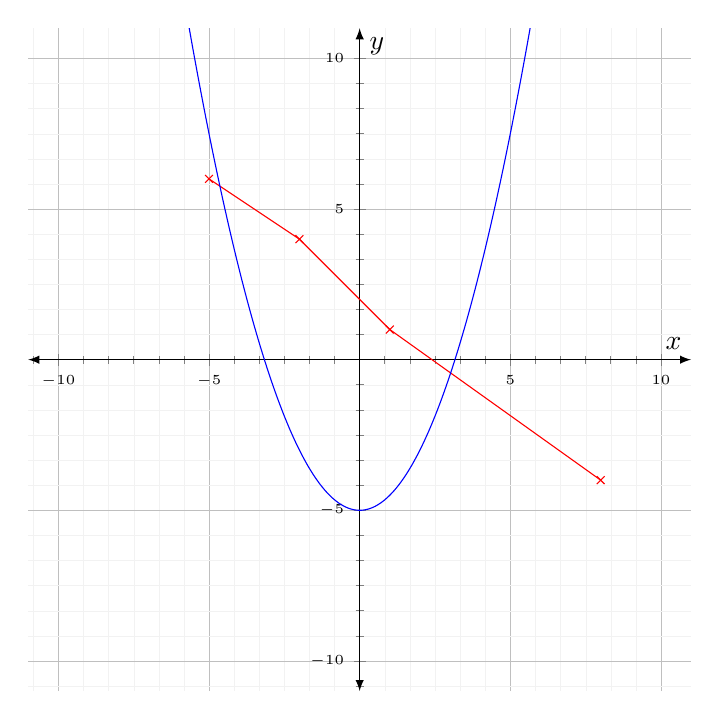
\begin{tikzpicture}
\begin{axis}[
	width=10cm,height=10cm,
	% WINDOW
    xmin=-11, xmax=11,
    ymin=-11, ymax=11,
    xlabel=$x$,ylabel=$y$,
    xlabel style={at={(ticklabel* cs:.975, 3)},anchor=north},
    ylabel style={at={(ticklabel* cs:.975, -3)},anchor=west},
    enlargelimits={abs=0.5},
    % GRID
    grid=both,
    grid style={line width=.1pt, draw=gray!10},
    major grid style={line width=.2pt,draw=gray!50},
    axis lines=middle,
    minor tick num=5,
    axis line style={latex-latex},
    ticklabel style={font=\tiny},
]
	\addplot[
		color=red,
		mark=x
	] coordinates {
		(-5,6)
		(-2,4)
		(1,1)
		(8,-4)
	};
	
	\addplot[
		color=blue,
		domain=-10:10,
		samples=100,
		smooth]
	{.5*x^2-5};
\end{axis}
\end{tikzpicture}
\end{document}